\section{Message Distribution System (MDS)}

\subsection{Sub topics}

\begin{itemize}
	\item Messaging distribution system - Why \& how?
	\item The PostOffice design - Why and how?
	\item Decoupling achieved.
	\item Design considerations \& implementation.
	\item Patterns per design and in relation to the MDS and PostOffice design:
	\begin{itemize}
		\item GoF Singleton Pattern
		\item GoF Observer Pattern
		\item GoF Mediator Pattern
	\end{itemize}
\end{itemize}

\subsection{Curriculum}

\begin{itemize}
	\item Slides: "A message system".
	\item OLA: "GoF Singleton pattern".
	\item OLA: "GoF Observer pattern".
	\item OLA: "GoF Mediator pattern".
\end{itemize}

\subsection{Exercises}

\begin{itemize}
	\item The Message Distribution System
\end{itemize}

\subsection{Message Distribution system - Why \& how?}

\subsubsection{Why?}
\begin{itemize}
	\item Lavere kobling.
	\begin{itemize}
		\item Subscriberne kan tilføje/fjerne sig selv, uden at publisheren skal tænke på det.
	\end{itemize}
	\item Lade subscriberne bestemmer selv hvad de vil have.
	\begin{itemize}
		\item Eksempelvis kan en graf subscribe på data til x og y, men ikke z.
	\end{itemize}
\end{itemize}

\subsubsection{How?}
\begin{itemize}
	\item Subscriberen sender følgende til MDS ved subscribtion:
	\begin{itemize}
		\item Hvilke data den vil subscribe på (Globalt).\todo{hvad mener der med globalt?}
		\item Pointer til egen MsgQueue.
		\item Local ID, som skal bruges når den skal modtage. \todo{vigtigheden af local id? tror måske jeg har en optagelse fra timen.. den lange og underlige snak.}
	\end{itemize}
	\item Ved opdatering på data \textit{x}, gør Publisher følgende:
	\begin{itemize}
		\item Finder alle der subscriber på \textit{x}.
		\item Sender data \textit{x} til subscribernes MsgQueue, med deres individuelle local ID.
	\end{itemize}
\end{itemize}

\todo{insert UML sekvensdiagram over kommunikation}

\subsection{The Postoffice Design - Why and how?}

\subsubsection{Why?}
Lavere kobling, som altid. Sender kender kun til modtagers navn og intet andet.

\subsubsection{How?}

\begin{itemize}
	\item Bruger navn på modtager.
	\begin{itemize}
		\item Sender skriver navn på modtageren.
		\item PostOffice finder den rigtige MsgQueue på baggrund af dette navn.
	\end{itemize}
	\item Bruger arv.
	\begin{itemize}
		\item Alle arver det samme enum af ID'er, som sendes med. \todo{not sure of meaning?}
	\end{itemize}
\end{itemize}

\todo{muligvis et klassediagram og/eller et sekvens?}

\subsection{Design considerations and implmentation.}
\todo{covered i det ovenfor? dunno..}

\subsection{Patterns per design and in relation to the MDS and Postoffice design}\todo{dobbelttjek at title navn er korrekt ift. eksamens spm}

\subsubsection{GoF Singleton Pattern}

Et singleton pattern er et software design pattern, der gør det muligt at begrænse antallet af instanser af en klasse til 1.

\paragraph{How to Singleton}

\begin{figure}[h]
	\centering
	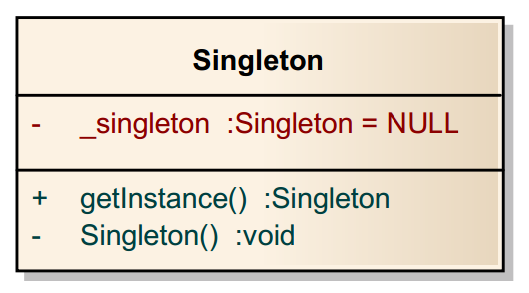
\includegraphics[width=0.4\linewidth]{figs/spm5/singletonclassdia}
	\caption{En Singleton klasse}
	\label{fig:SingletonClass}
\end{figure}

\begin{itemize}
	\item Private constructor - Sikrer at kun klassen kan oprette en instans, ingen andre kan oprette eller kopiere den!
	\item statisk \textit{getInstance()} funktion - Statisk så den kan kaldes uden et objekt. Denne funktion returnerer instansen, og laver en ny hvis den private pointer (instansen) til sig selv er NULL.
	\item Statisk private pointer til sig selv - Den eneste instans\todo{right??}.
\end{itemize}

\paragraph{Singleton pattern i forhold til MDS og postoffice design}
\todo{her skal der være noget med øvelsen}

\subsubsection{GoF Observer Pattern}

Et GoF observer pattern, også kaldet Publisher/Subscriber pattern består af to primære elementer:

\begin{itemize}
	\item Publisher (subject) - Kan have flere subscribere(observere) der abonnerer på den.
	\item Subscriber (observer) - Bliver notificeret når publisher ændrer state. Herefter anmodes publisher om faktiske æmdringer.
\end{itemize}

Dette pattern er brugbart når ændringer i et objekt kræver ændring i andre, og hvor man ikke ved hvilke og hvor mange der er tale om.

\begin{figure}[h]
	\centering
	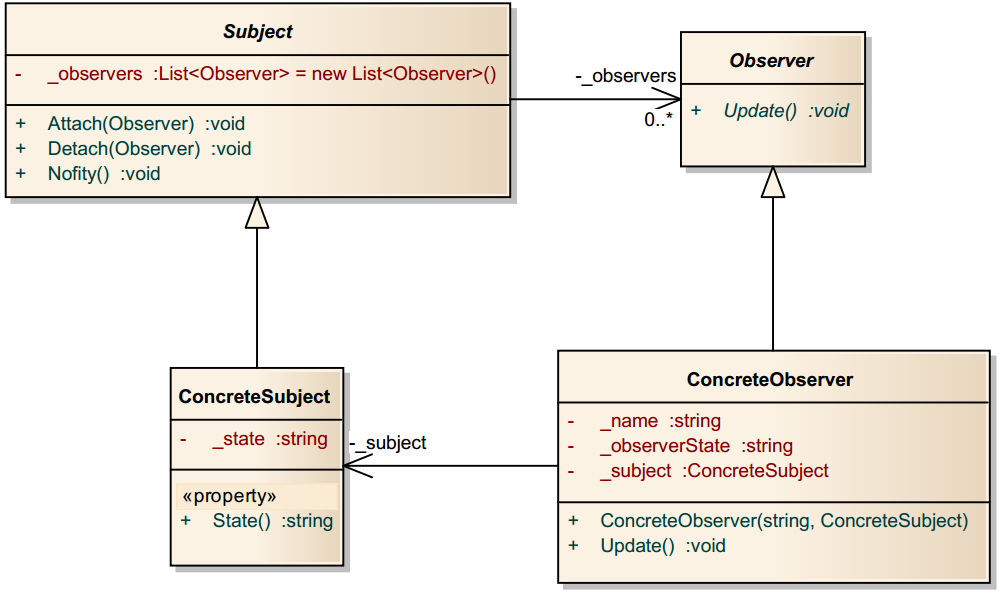
\includegraphics[width=0.8\linewidth]{figs/spm5/observerUML}
	\caption{Et Observer pattern, konfigureret til \textit{pull}.}
	\label{fig:ObserverPattern}
\end{figure}

\paragraph{Observer pattern i forhold til MDS og postoffice design}
\todo{her skal der være noget med øvelsen}

\subsubsection{GoF Mediator Pattern}
Når objekters funktionalitet distribueres ud mellem hinanden, vil der opstå høj kobling, og masser af interkonnektivitet.  I et mediator pattern oprettes et separat mediator-objekt, som står for at kontrollere objekters interaktioner med hinanden. 

\paragraph{Løsning}

\begin{figure}[h]
	\centering
	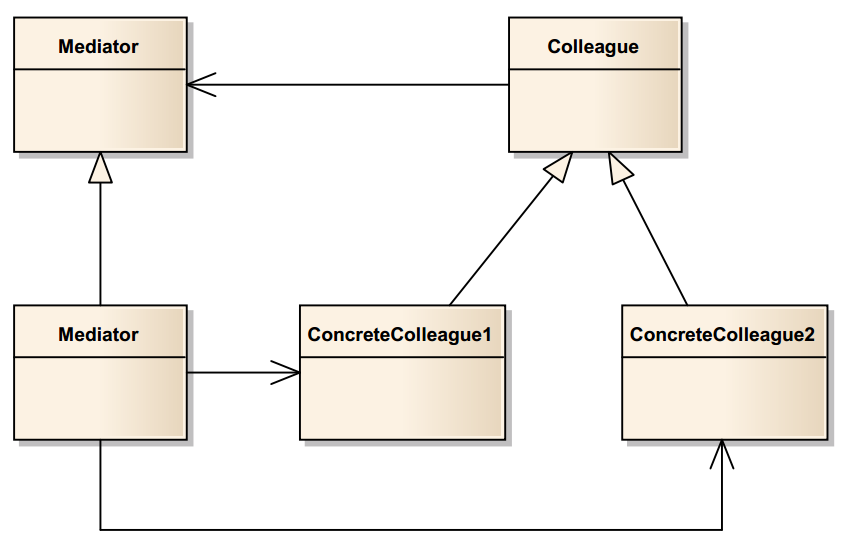
\includegraphics[width=0.8\linewidth]{figs/spm5/concrete}
	\caption{Generelt klassediagram om Mediator pattern.}
	\label{fig:concrete}
\end{figure}

Definition og identifikation af deltagende klassers type:

\begin{itemize}
	\item Mediator.
	\begin{itemize}
		\item 	Definerer et interface til kommunikation med “Colleague objekter”.
	\end{itemize}
	\item Concrete mediator.
	\begin{itemize}
		\item 	Implementerer kommunikationsinterfacet, ved at koordinere Colleague objekter.
	\end{itemize}
	\item Colleague klasser.
	\begin{itemize}
		\item Hver colleague klasse kender sit mediator object.
		\item Når colleaguen vil snakke med en anden klasse, kommunikeres der udelukkende gennem mediatoren.
	\end{itemize}
\end{itemize}

Brugen af et mediator pattern begrænser mængden af afledte klasser i et system, i og med mediatoren centraliserer funktionalitet der ellers ville være spredt ud på mange klasser. Ved at pakke objekters interkonnektivitet ind i et mediator pattern, får man samtidig skabt et ekstra abtraktionsniveau der gør funktionalitet mere overskuelig.

\paragraph{Sammenligning}
Mediator patternet kan sammenlignes med \textbf{publisher-subscriber}. Begge står for at håndtere kommunikationen mellem to eller flere klasser. Hvor publisher-subscriber blot broadcaster til alle subscribers, så har mediatoren i højere grad funktionalitet til at finde ud af, hvilke "colleague" eller "subscribers" der skal udføres noget på. Wiki har et glimrende eksempel på siden om Mediator, som viser, at alt efter hvilken kommando der kaldes, så udfører mediatoren noget forskelligt, og kalder metoderne hos de registrerede objekter med forskellige parametre.

\paragraph{Konsekvenser}
Mediatoren samler en masse funktionalitet på ét sted, hvilket har den fordel at interaktionen mellem objekter bliver nemmere, men mediatoren får derved større ansvar og bliver mere kompleks. Mediatoren kan derfor hurtigt blive en monolit, som er svær at vedligeholde.\\

Mediator pattern er godt at bruge, i tilfælde, hvor der opstår mange forbindelser mellem mange forskellige klasser. Ved hjælp af mediatoren centraliseres referencerne til de forskellige objekter ét sted, og samler kald til mediatoren, i stedet for enkelte klasser. Dog skal der passes på at mediatoren ikke bliver til en monolit, hvis for meget funktionalitet bliver pakket ind i den.
